\documentclass{article} %  say
\usepackage{tikz}
\begin{document}
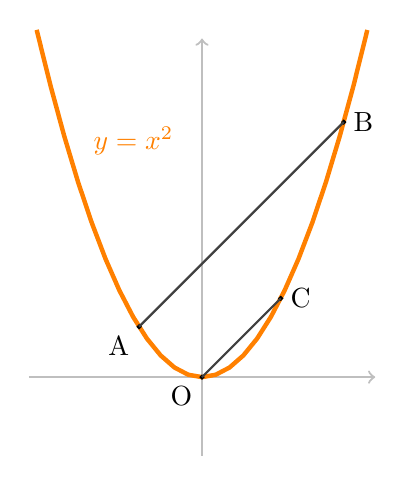
\begin{tikzpicture}[scale=1]
  
  %\draw[step=.5cm,gray,very thin] (-1.4,-1.4) grid (1.4,1.4);
  %\draw[help lines] (-2,-1) grid (2,4);
  
  % x axis
  \draw [lightgray, thick, ->] (-2.2,0) -- (2.2,0);
  
  % y axis
  \draw [lightgray, thick, ->] (0,-1) -- (0,4.3);
  
  % plot y=x^2
  \draw[orange, ultra thick, domain=-2.1:2.1] plot (\x, {\x*\x});
    
   % label A
  \draw[fill] (-0.8,0.64) circle [radius=0.025];
  \node [below left] at (-0.8,0.64) {A};
  
  % label B
  \draw[fill] (1.8,3.24) circle [radius=0.025];
  \node [right] at (1.8,3.24) {B};
  
  %line AB
   \draw [darkgray, thick] (-0.8,0.64) -- (1.8, 3.24);

 % label O
  \draw[fill] (0,0) circle [radius=0.025];
  \node [below left] at (0,0) {O};
  
  % label C
  \draw[fill] (1,1) circle [radius=0.025];
  \node [right] at (1,1) {C};
  
 %line OC
  \draw [darkgray, thick] (0,0) -- (1, 1);

  % plot title
  \node [right, orange] at (-1.5,3) {$y=x^2$};
  
\end{tikzpicture}
\end{document}